\chapter{Theoretical Background}
\label{chap:Theory}
Since 1930s, many theories and discoveries in particle physics have revealed the fundamental structure of matter. The matter is made up of fundamental particles and their interactions are mediated by four fundamental forces \cite{Griffiths:111880}. The theoretical models describe all the phenomena of particle physics as well as predict the nature and properties of particles. These models must be either confirmed experimentally or totally excluded giving hints of new physics. This interplay between experimental discoveries and the corresponding theoretical predictions leads to describe the fundamental particles and their interactions through a theoretical model, known as the Standard Model. The world's most powerful particle accelerators and detectors are used by physicists to test the predictions and limits of the Standard Model where it has successfully explained almost all experimental results. This chapter describes the Standard Model with the main focus on Quantum Chromodynamics and its properties which serve as the theoretical foundations of this thesis.

%The growing knowledge about fundamental and new particles was accompanied by the evolution of quantum mechanics and the special relativity. 
\section{Standard Model}
The Standard Model (SM) of particle physics \cite{Perkins:1982xb,Herrero:1998eq,Weinberg:1967tq} was developed in 1970s. It is a mathematical framework which describes the properties of fundamental particles and the forces of interactions between them, as summarized in Fig.~\ref{fig:SM}. According to the SM, there are 12 elementary particles i.e. without any internal structure, known as fermions. The fermions having half integral spin obeying Fermi-Dirac statistics and follows the Pauli exclusion principle. Each fermion has a corresponding antiparticle with same properties but opposite-sign quantum numbers.
\begin{figure}[!h]
\begin{center}
\hspace*{-15mm}
%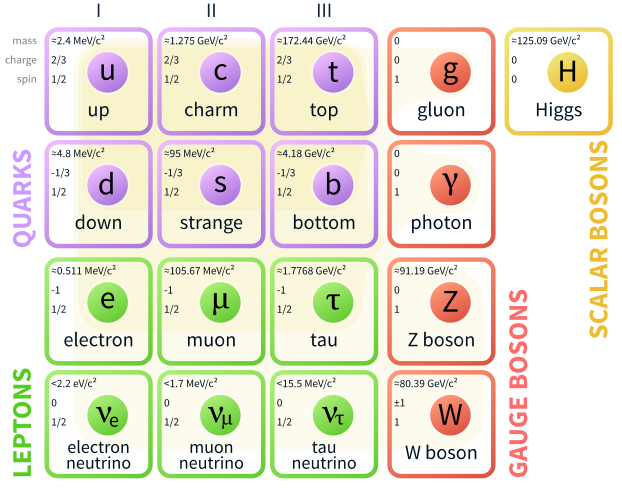
\includegraphics[scale = 0.8]{/home/anter/Desktop/Thesis/Figures/StandardModel_edited.png}\\
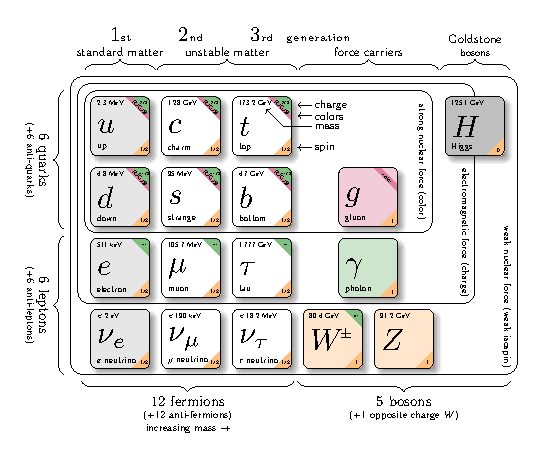
\includegraphics[width=1.2\textwidth]{/home/anter/Desktop/Thesis/Figures/model-physics.pdf}\\
%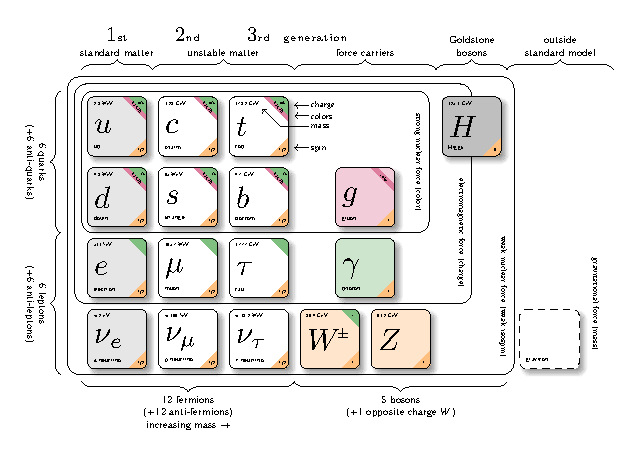
\includegraphics[width=1.2\textwidth]{/home/anter/Desktop/Thesis/Figures/original_model-physics.pdf}\\
\caption[SM]{The Standard Model\footnotemark summarizing the properties of elementary particles known as fermions (leptons and quarks), grouped into three generations, gauge bosons as mediators for the interactions, the scalar Higgs boson and not corporated graviton for the gravitational force.}
\label{fig:SM}
\end{center}
\end{figure}
\footnotetext{Source : \url{http://www.texample.net/tikz/examples/model-physics}}%https://en.wikipedia.org/wiki/Standard_Model}}
Depending on how the fermions interact, they are classified into two categories - leptons (\sln) and quarks ($q$). There are six types of leptons : electron ($e$), muon ($\mu$) and tau ($\tau$) with electric charge Q = -1 (all charges are in the units of elementary charge $e$) and the corresponding neutrinos $\nu_e$, $\nu_\mu$ and $\nu_\tau$ having electric charge Q = 0. There are six ``flavors'' of quarks : up ($u$), down ($d$), strange ($s$), charm ($c$), bottom ($b$) and top ($t$). $u$, $c$ and $t$ carry charge Q = $\pm$ $\frac{2}{3}$ whereas $d$, $s$ and $b$ carry charge Q = $\pm$ $\frac{1}{3}$. The quarks and leptons are categorized into three generations. The lightest and the most stable particles belong to first generation and the second and third generations have the heavier and less stable particles.

There are four fundamental forces existing in nature : electromagnetic, strong, weak and gravitational force. Every interaction involves the exchange of a gauge boson : the photon ($\gamma$) for the electromagnetic force, gluons ($g$) for the strong force, two $W$'s and a $Z$ for the weak force and the graviton (not yet found) for the gravitational force. However, the gravitational force has not been incorporated into SM yet. Along with this, the existence of dark matter or energy and the matter-antimatter asymmetry are still missing pieces in the SM. Each force acts between particles because of some property of that particle - charge for electromagnetism, color for the strong force and flavor for the weak force. 

In the SM, first three forces are unified into one quantum field theory \cite{Peskin:1995ev}, known as Grand Unified Theory (GUT) \cite{Glashow:1979pj,Salam:1980jd,Georgi:1974sy}. The SM framework is based on quantum field theories and is described by SU(3)$_{\rm C}~\otimes$ SU(2)$_{\rm L}~\otimes$ U(1)$_{\rm Y}$ gauge symmetry. Here, SU(2)$_{\rm L}~\otimes$ U(1)$_{\rm Y}$ term describes the weak and electromagnetic forces, respectively. The electromagnetic interaction of particles is explained by a well established modern theory of Quantum Electrodynamics (QED). In SM, the weak and electromagnetic interactions are combined by electroweak theory. The electroweak symmetry is spontaneously broken by the coupling to the scalar Higgs field. The gauge bosons of the unified electroweak theory are a mixture of the gauge bosons of the unbroken symmetry resulting in the massive $W^{\pm}$ and $Z$ bosons, and the massless photon ($\gamma$). The Higgs boson, named after Peter Higgs, is the field quantum of the Higgs field responsible for electroweak symmetry breaking. It was discovered by the CMS \cite{Chatrchyan:2012xdj} and ATLAS \cite{Aad:2012tfa} collaborations in 2012, with the properties consistent with the SM. The SU(3)$_{\rm C}$ term defines the strong interaction between quarks and gluons mediated by gluons, with the three degrees of freedom of the color charge (C). In contrast to the electroweak symmetry, the SU(3)$_{\rm C}$ of the strong interaction is an exact symmetry and hence the gluons are massless. The strong interaction between quarks and gluons is described by theory called Quantum Chromodynamics (QCD), explained in details in the next section of this thesis.

\section{Quantum Chromodynamics}
Quantum Chromodynamics \cite{Ellis:1991qj, Halzen:1984mc} is the non-abelian gauge theory of strong interactions between the quarks and gluons. The gauge group of QCD is the special unitary group SU(3)$_{\rm C}$ with color charges C as the generators of the gauge group. Color charge is the peculiar property of QCD and has a same role as the electric charge in electromagnetic interactions. However, the mediator of electromagnetic interactions i.e. photon, itself does not carry any electric charge where as the gluon carry color charge. This allows the self coupling of gluons and hence make the theory non-Abelian. Both the quarks and gluons carry three colors : red ($r$), green ($g$) and blue ($b$), and three anti-colors : anti-red ($\bar{r}$), anti-green ($\bar{g}$) and anti-blue ($\bar{b}$). The quarks carry a single color charge whereas gluons carry a combination of color charges. There are nine eigen states of gluons but one of them $\frac{1}{\sqrt{3}}(r\bar{r}~\plus g\bar{g}~\plus b\bar{b})$ is totally symmetric color singlet which has no net color charge and does not take part in interaction. The remaining eight eigen states of the gluons are :
\begin{equation}
r\bar{b},~r\bar{g},~b\bar{g},~b\bar{r},~g\bar{r},~g\bar{b},~\frac{1}{\sqrt{2}}(r\bar{r}~-~b\bar{b}),~\frac{1}{\sqrt{6}}(r\bar{r}~\plus b\bar{b}~-~2g\bar{g}) 
\end{equation}

The dynamics of the quarks and gluons are controlled by the gauge invariant QCD Lagrangian $\mathcal{L}_{QCD}$ which is composed of four terms as : 
\begin{equation}
\mathcal{L}_{QCD} = \underbrace{-\frac{1}{4}F^A_{\mu\nu}F^{\mu\nu}_A}_\text{$\mathcal{L}_{gluons}$}~\plus \underbrace{\sum\limits_{flavors}^{} \bar{q}_a \big(i\gamma^\mu (D_\mu)_{ab}~-~m_q\big)q_b}_\text{$\mathcal{L}_{quarks}$}~\plus \mathcal{L}_{gauge}~\plus\mathcal{L}_{ghost}
\label{eq:lag}
\end{equation}
where $\mathcal{L}_{gluons}$ represents the kinetic term of the gluon fields ${\cal A}^A_\mu$, $\mathcal{L}_{quarks}$ describes the interaction of spin-$\frac{1}{2}$ quark fields $q_a$ of mass $m_q$ with spin-1 gluon fields ${\cal A}^A_\mu$ summing over all presently known six flavors u, d, s, c, b, and t; $\mathcal{L}_{gauge}$ defines the chosen gauge and $\mathcal{L}_{ghost}$ is the so-called ghost term which is a remedy necessary to treat the degeneracy of equivalent gauge field configurations in non-Abelian gauge theories. Here the Greek letters $\mu$, $\nu$, ... $\in$ \{0,1,2,3\} represents space-time indices whereas a,b,c $\in$ \{1,2,3\} and A,B,C $\in$ \{1,...,8\} are the indices of the triplet and octet representations, respectively, of the SU(3)$_{\rm C}$ gauge symmetry group. $F^A_{\mu\nu}$ is the field tensor defined as
\begin{equation}
F^A_{\mu\nu} = \partial_\mu {\cal A}^A_\nu - \partial_\nu {\cal A}^A_\mu - g_s f_{ABC}{\cal A}^B_\mu {\cal A}^C_\nu
\label{eq:field}
\end{equation}
where $g_s$ is the coupling constant determining the strength of the interaction between colored partons and $f_{ABC}$ are the structure constants of the SU(3)$_{\rm C}$ group. The third term in Eq.~\ref{eq:field} is a non-Abelian term which distinguishes QCD from QED and gives rise to a three-gluon and a four-gluon vertex. ($D_\mu$)$_{ab}$ is the covariant derivative given by Eq.~\ref{eq:cov} and $\gamma_\mu$ are the Dirac $\gamma$-matrices. 
%In the second term of Eq.~\ref{eq:lag}, 
\begin{equation}
(D_\mu)_{ab} = \partial_{\mu}\delta_{ab}~\plus ig_sT^A_{ab}{\cal A}^A_\mu
\label{eq:cov}
\end{equation}
There are eight gluon fields ${\cal A}^A_\mu$ with factors $T^A_{ab}$ corresponding to the generators of the SU(3)$_{\rm C}$ gauge group. A representation of the generators is given via $T^A$ = $\lambda^A$/2 by the Hermitian and traceless Gell-Mann matrices $\lambda^A$ \cite{GellMann:1962xb}. The generator matrices $T^A$ satisfy the commutation relations 
\begin{equation}
\bigg[T^A,T^B\bigg] = if_{ABC}T^C
\end{equation}

In $\mathcal{L}_{QCD}$, the classical contribution comes from $\mathcal{L}_{gluons}$ and $\mathcal{L}_{quarks}$ terms which correspond to the free quark- and gluon-field terms, and the quark-gluon interaction term presented in Fig.~\ref{fig:feyn}. Along with this, the non-Abelian group structure of QCD leads to the cubic and quartic gluon self-interaction vertices, which are proportional to $g_s$ and $g^2_s$, respectively.

\begin{figure}[!h]
\begin{center}
\hspace*{-1mm}
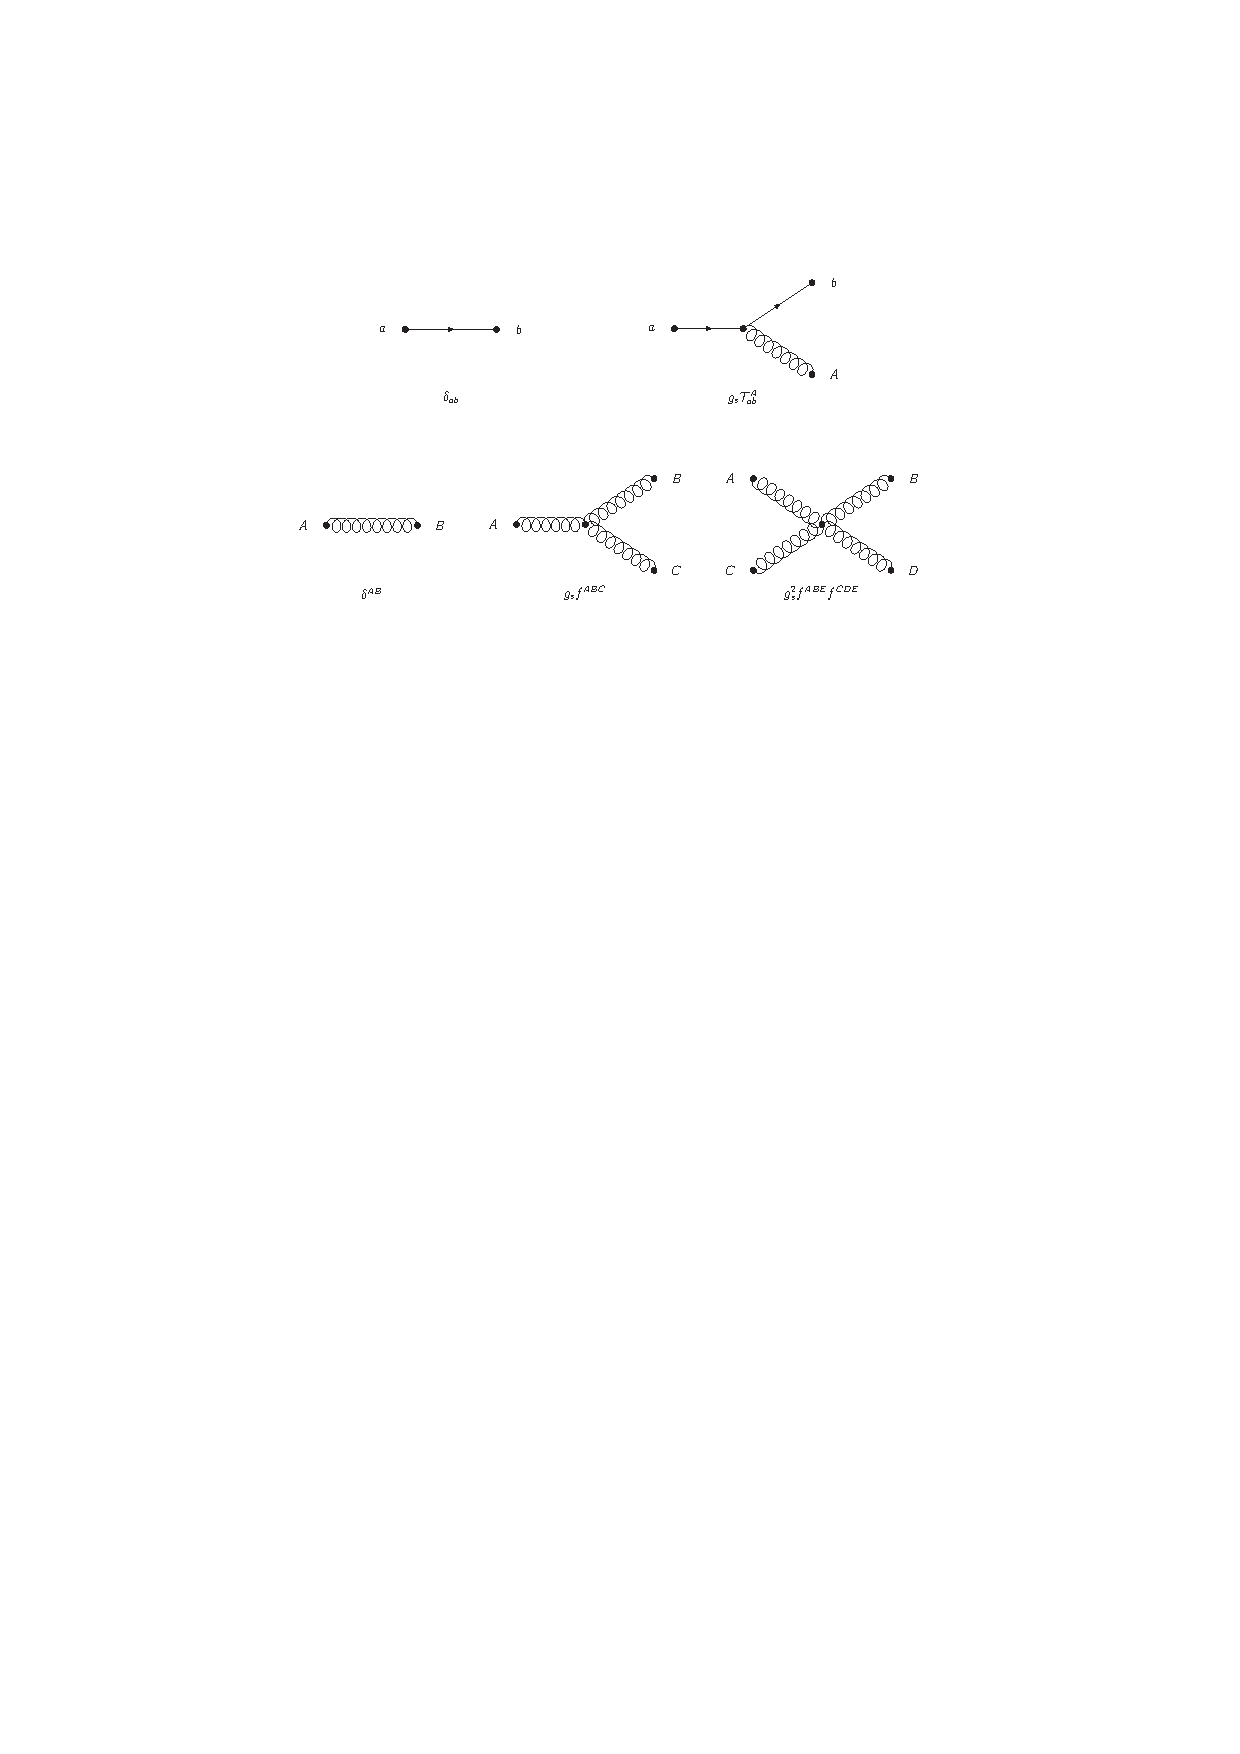
\includegraphics[width=0.95\textwidth]{/home/anter/Desktop/Thesis/Figures/edited_cropped_Feynmann.pdf}\\
\vspace*{4mm}
\caption{The fundamental Feynman rules of a free quark-field term (top left), quark-gluon interaction term (top right), free gluon-field term (bottom left), cubic gluon self-interaction term (bottom middle) and quartic gluon self-interaction term (bottom right). Taken from \cite{Rabbertz:2017ssq}.}
\label{fig:feyn}
\end{center}
\end{figure}

It is impossible to use perturbation theory on a gauge invariant Lagrangian without choosing a specific gauge in which to calculate. The usual gauge-fixing term is given by 
\begin{equation}
{\cal L}_{gauge}=-\frac{1}{2\xi} (\partial^{\mu}{\cal A}^{A}_{\mu})^{2}
\label{eq:gauge-fixing}
\end{equation}
where $\xi$ may be any finite constant. This choice fixes the class of covariant gauges with $\xi$ as the gauge parameter. As QCD is non-Abelian, the gauge fixing term must be supplemented by a ghost Lagrangian as
\begin{equation}
{\cal L}_{ghost}=\partial_{\alpha}\eta^{A\dagger}(D^{\mu}_{AB}\eta^{B})
\label{eq:ghost}
\end{equation}
where $\eta^{A}$ is a complex scalar field which obeys Fermi statistics. The ghost fields cancel unphysical degrees of freedom which arise due to using covariant gauges. This completes the QCD Lagrangian shown in equation \ref{eq:lag}.

The strength of an interaction is given by a fundamental parameter called the coupling constant $\alpha$. In QED, the coupling constant $\alpha_e$ = $e^2/4\pi$ = 1/137 is constant. In contrast to this, in QCD, the coupling constant \alpsq = $g^2_s/4\pi$ is not constant and depends on the separation between the interacting particles. It increases with the increase in the distance or decrease in the energy scale Q. At large distances or low energies, the quarks can never be found as free particles but as color neutral bound states called hadrons. Hadrons are of two types : baryons and mesons made up of quark-antiquark pair and ($qqq$) made from three (anti-)quarks. According to the quark model \cite{Griffiths:111880} every (anti-)baryon is made up of three (anti-)quarks and every meson is composed of a quark and an antiquark. When the colored quarks and gluons within a hadron are pulled farther and farther apart, there is an increase in the strength of force between them. This results in creation of new quark-antiquark pair making difficult to liberate a free quark or gluon. This property of QCD is known as confinement. As it would take an infinite amount of energy to separate two quarks, they are forever bound into hadrons such as protons ($uud$), neutrons ($udd$). Although the gluons are massless, the confinement leads to the finite range of the strong interactions. On the other hand, at small distances, the quarks and gluons interact very weakly and are treated as free particles. This property is known as asymptotic freedom. This indicates that perturbation theory is only applicable at high energies or small distances.

\subsection{Perturbative Quantum Chromodynamics}
At high energies, the property of asymptotic freedom allows a perturbative treatment in QCD calculations. In perturbative Quantum Chromodynamics (pQCD), any observable $X$ such as cross-section of a scattering process, can be written as a perturbative series in terms of coupling constant \alps as : 
\begin{equation}
X = \sum\limits_{i=0}^{N} \alpha^n_s {\rm c}_i = {\rm c}_0~\plus \alpha^1_s {\rm c}_1~\plus \alpha^2_s {\rm c}_2~\plus ...
\end{equation} 
where ${\rm c}_i$ are the perturbative coefficients. In a process, the pQCD calculation of X is determined by over the amplitudes of all Feynman diagrams. For a given Feynman diagram, the power of \alps is determined by the number of vertices associated with quark-gluon or gluon-gluon interactions. A leading order (LO) prediction sums over only the lowest-order contribution whereas next-to-leading order (NLO) includes terms with an additional powers of \alps. The next-next-to-leading order (NNLO) includes emission of another gluon or a virtual gluon loop. The different order of the QCD processes are shown in Fig.~\ref{fig:orders}.
\begin{figure}[!h]
\begin{center}
\hspace*{-1mm}
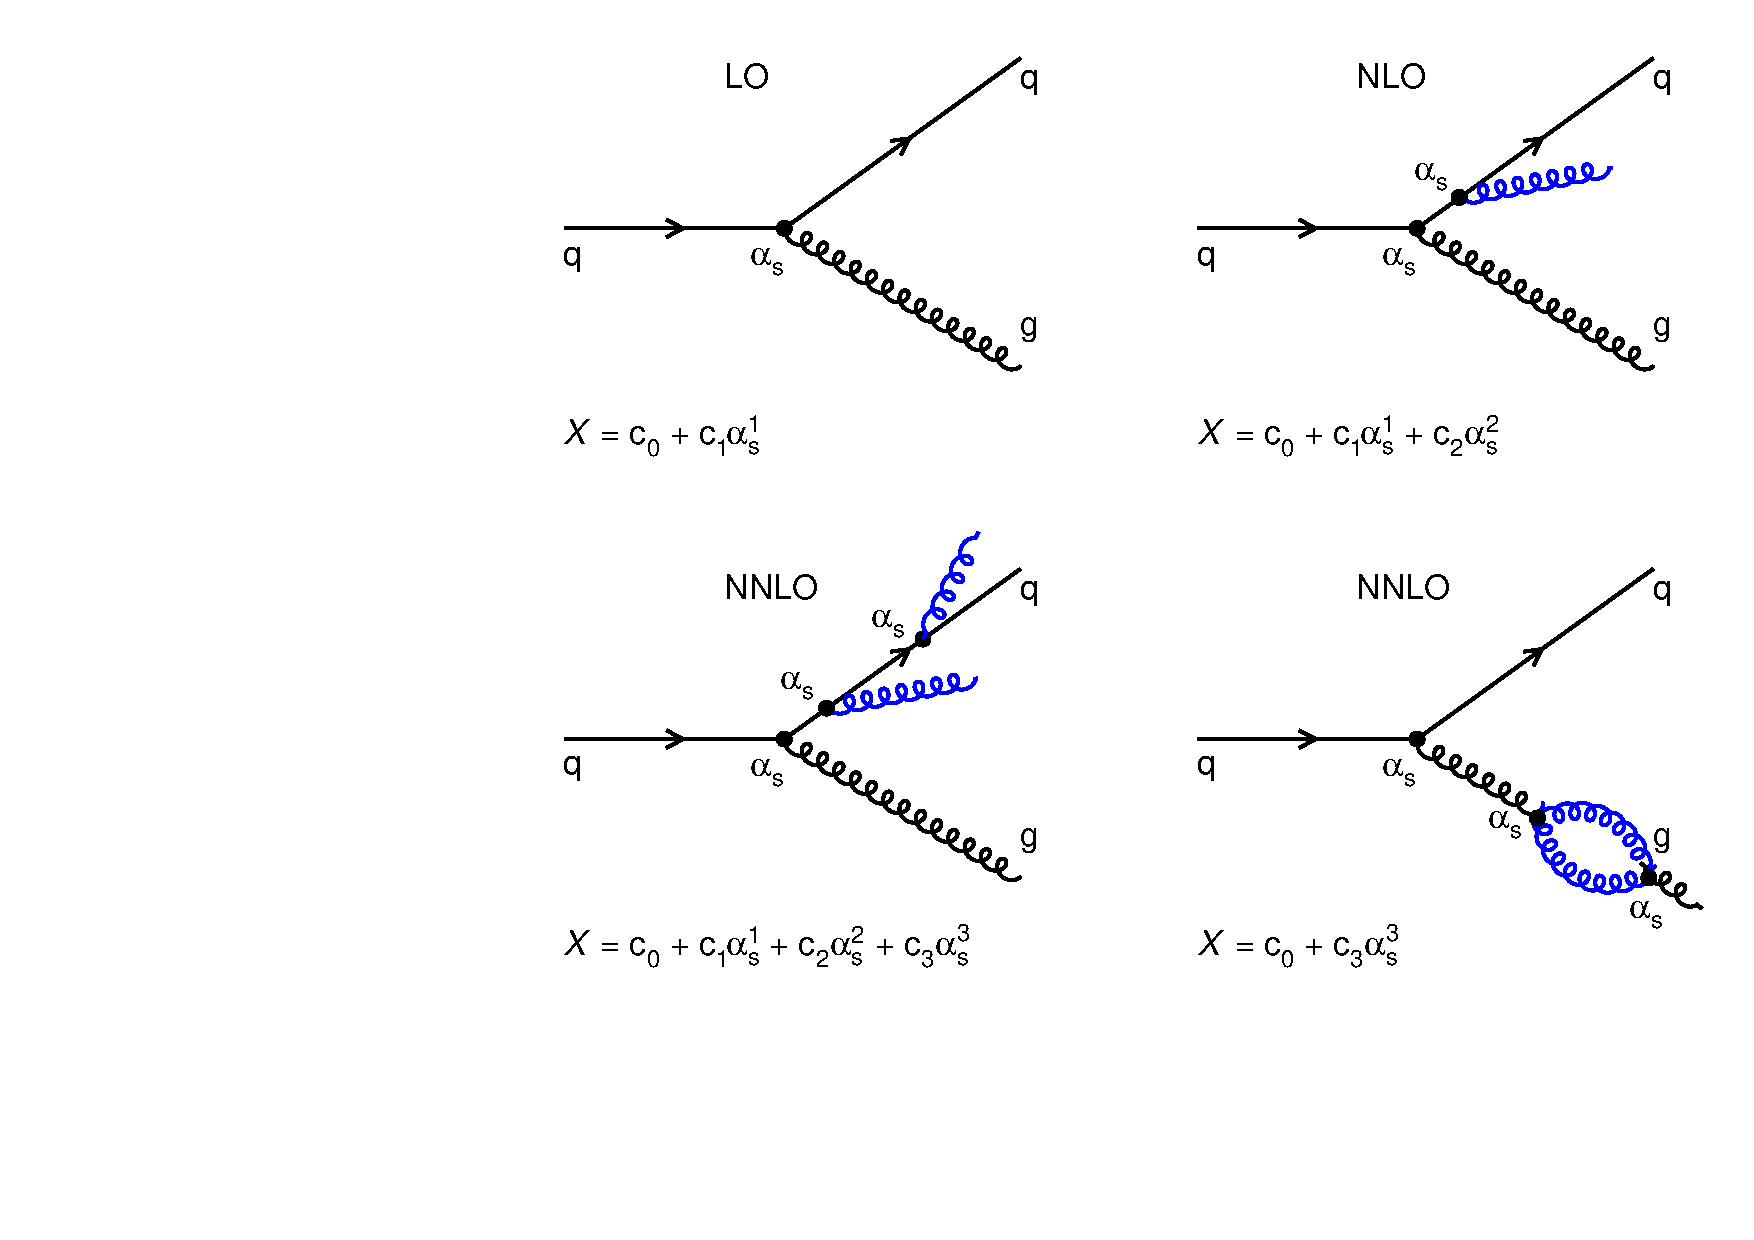
\includegraphics[width=0.95\textwidth]{/home/anter/Desktop/Thesis/Figures/Orders.pdf}\\
\vspace*{4mm}
\caption[Feyn]{Feynman diagrams\footnotemark showing leading-order (LO), next-to-leading order (NLO) and next-next-to-leading order (NNLO) processes in QCD along with the perturbative expansion of any observable $X$ in powers of the strong coupling constant \alps. At each successive step in perturbation series, the emission of an additional gluon take place.}
\label{fig:orders}
\end{center}
\end{figure}
The calculations become complex with the loop diagrams where the momenta of the virtual particles in a loop are not fully constrained by four-momentum conservation and the associated integrals are divergent. Such ultraviolet (UV) divergencies enter the calculations beyond LO due to loop or vertex corrections. These are overcome by a procedure known as renormalization, described in next Section. Apart from these, QCD also suffers from infrared and collinear divergences (IRC) due to the presence of massless gluons and neglected quark masses. These need to be handled in pQCD calculations. The observable to be studied must be IRC safe. 

\subsection{Renormalization and Running of the Strong Coupling}
The renormalization is a mathematical procedure which allows the finite calculation of momenta integrals of loop by removing UV divergences. \footnotetext{Drawn using ROOT}It introduces a regulator for the infinities, the renormalization scale \mur. At first, the divergences are regularized temporarily by introducing a cut-off to the loop momenta at \mur scale. Then the free parameters of the Lagrangian, i.e. the coupling constant are redefined (renormalized) to absorb the UV divergences. Hence, both \alpsq and observable $X$ become a function of \mur. The exact dependence of \alpsmusq on \mur is described by the renormalization group equation (RGE), which determines the running of \alpsmusq. RGE states that the dependence of $X$ on \mur must cancel, which is expressed mathematically as : 
\begin{equation}
\mur^{2}\frac{d}{d\mur^{2}}X\Bigg(\frac{Q^{2}}{\mur^{2}},\alpha_{s}(\mur^{2})\Bigg)=
\Bigg(\mur^{2}\frac{\partial}{\partial\mur^{2}}~\plus \mur^{2}\frac{\partial\alpha_{s}(\mur^{2})}
{\partial\mur^{2}}\frac{\partial}{\partial\alpha_{s}(\mur^{2})}\Bigg)X=0
\label{eq:dmu}
\end{equation}
Using $\beta(\alps)$ = $\mur^{2}\frac{\partial\alpha_{s}(\mur^{2})}{\partial\mur^{2}}$, Eq.~\ref{eq:dmu} can be re-written as 
\begin{equation}
\Bigg(\mur^{2}\frac{\partial}{\partial\mur^{2}}~\plus \beta(\alps)\frac{\partial}{\partial\alpha_{s}(\mur^{2})}\Bigg)X=0
\label{eq:dmu2}
\end{equation}
By setting the renormalization scale to the physical scale i.e. $Q^{2}=\mu^{2}$, $X(1,\alpha_{s}(Q))$ is a solution to above equation. $Q$-dependence of the $X$ is only from the renormalization of the theory and would not be present in the classical theory. Hence measuring the $Q$-dependence of $X$ will directly probe the quantum structure of the theory. The $\beta$ function in QCD has a perturbative expansion as : 
\begin{equation}
\beta(\alps)=-\alpha_{s}^{2}\Big(b_0~\plus b_1\alps~\plus b_2\alpha_{s}^{2}~\plus {\cal O}(\alpha_{s}^{3})\Big) 
\label{eq:beta}
\end{equation}
where $b_0$, $b_1$ and$b_2$ are the 1-loop, 2-loop and 3-loop $\beta$-function coefficients encoding the dependence of the coupling on the energy scale and given in the modified minimal subtraction ($\overline{\rm MS}$) scheme \cite{tHooft:1973mfk,Weinberg:1951ss} as :
\begin{equation}
b_0 = \frac{33-2n_f}{12\pi}, ~~~b_1 = \frac{153-19n_f}{24\pi^2}, ~~b_2 = \frac{77139 - 15099n_f~\plus 325n^2_f}{3456\pi^3}
\end{equation}
where $n_f$ is the number of quark flavours with masses $m_q$ smaller than the scale \mur. On integration of above equation, the energy dependence of \alps is yielded. Neglecting the higher orders, the first order solution of RGE is :
\begin{equation}
\alpha_{s}(\mur^2)=\frac{1}{b_0~{\rm ln}(\mur^2/\Lambda^2_{QCD})}
\label{eq:sol}
\end{equation}
with $\Lambda_{QCD}$ as the constant of integration. It corresponds to the scale at which the perturbative coupling would become large and the perturbative series diverge. With $b_0$ \gr 0, the coupling becomes weaker at higher scales $Q$, i.e. the effective color charge gets smaller when the distance decreases. This allows the quarks to behave as free particles within the hadron, leading to the property called asymptotic freedom. It is convenient to express \alps at some fixed scale. As some of the best measurements come from $Z^0$ decays, it is common practise to give the strong coupling at the scale of the $Z$ boson mass as \alpsmz. So, Eq.~\ref{eq:sol} can be expressed as :
\begin{equation}
\alps\big(\mur,\alpsmz\big) = \frac{\alpsmz}{1\plus\alpsmz b_0{\rm ln}(\mur^2/M^2_z)}
\end{equation}

The free parameter \alps of the theory is deduced from experimental measurements and evolved to the scale of the $Z$ boson. The current world average value of the strong coupling constant according to the PDG \cite{Patrignani:2016xqp} is 
\begin{equation}
\alpsmz = 0.1181 \pm 0.0011
\end{equation}
This value is derived using hadronic $\tau$ lepton decays, lattice QCD calculations, deep inelastic scattering data, electron-positron annihilation processes and electroweak precision fits. The various determinations of the strong coupling constant at scale $Q$, describing the running of the strong coupling up to the 1 TeV scale, are shown in Fig.~\ref{fig:alpha_pdg}.

\begin{figure}[!h]
\begin{center}
\hspace*{-7mm}
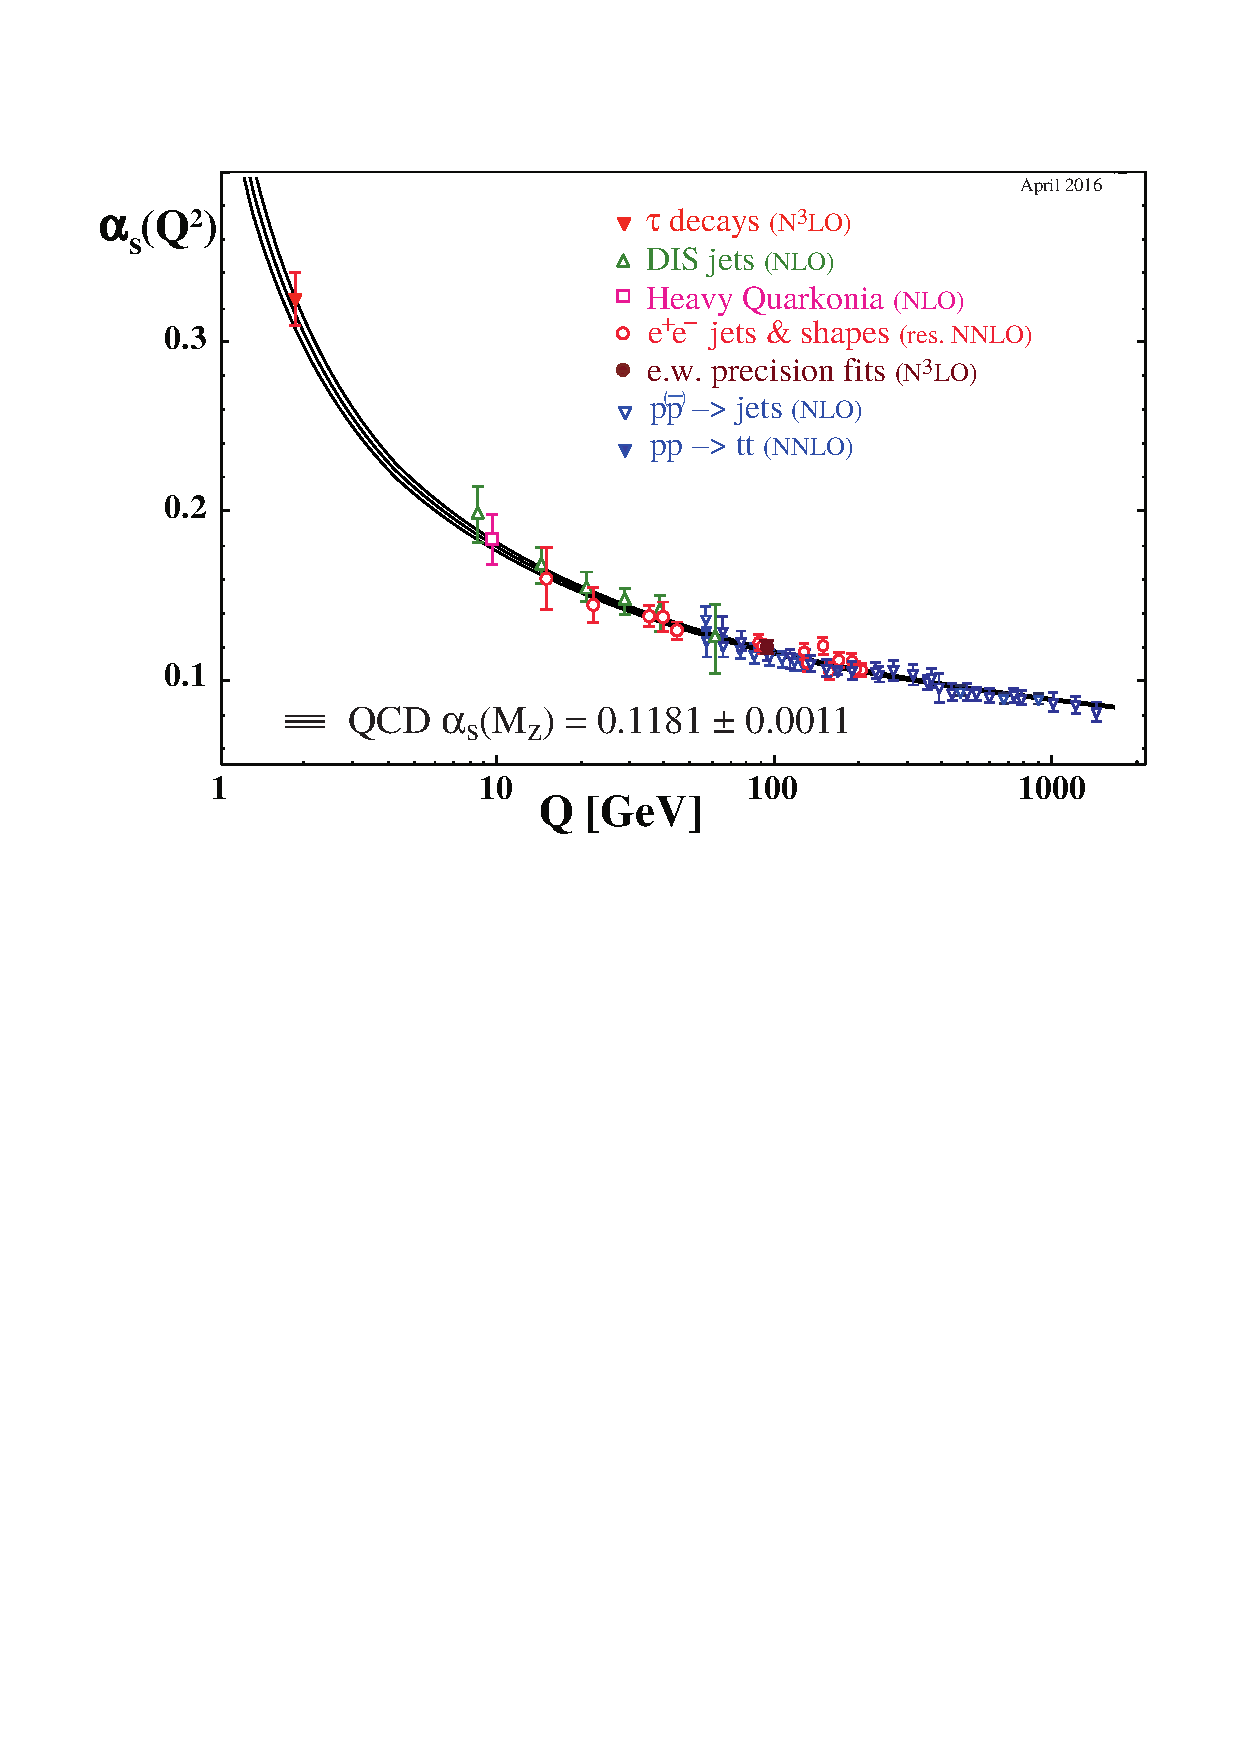
\includegraphics[width=0.95\textwidth]{/home/anter/Desktop/Thesis/Figures/cropped_Alpha.pdf}\\
\vspace*{4mm}
\caption[PDG]{The measurement of the strong coupling constant \alps as a function of the energy scale $Q$ from various experiments is are shown. These describe the running of the \alps up to the 1 TeV scale. Taken from ~\cite{Patrignani:2016xqp}.}
\label{fig:alpha_pdg}
\end{center}
\end{figure}

\section{Hadronic Collisions}

The collision between two hadrons is visualized as an interaction between their constituents, known as partons - quarks and gluons, at at a large momentum transfer, $Q$. At the Large Hadron Collider (LHC), the hadrons involved in the collisions are protons : a complex composite particles consisting of three valence quarks ($uud$) and gluons for the exchange of the strong force. The proton also contains `sea quarks' consisting of quark-anti-quark pairs coming into and out of existence rapidly and continuously due to gluon colour field splitting. In a collision, one of the most important quantities to evaluate is the cross-section ($\sigma$) of a certain process. It gives the probability that the two hadrons interact and give rise to that specific process. But in a hadronic collision, the perturbation theory is only valid at the parton-level and due to property of confinement at low energies, free partons cannot exist in nature. Only hadrons having a complex internal structure are available for the high energy collisions. So, a factorization theorem of QCD \cite{Collins:1989gx} comes into play which allows the calculation of $\sigma$ by separating into two parts : a short-distance partonic cross-section calculable with pQCD, and a non-perturbative long-distance part described by parton distribution functions (PDFs) $f_i(x,\muf)$. \muf is a factorization scale which corresponds to the resolution with which the hadron is being probed. The particles emitted with transverse momenta above \muf are considered in the hard scattering perturbative coefficients whereas those emitted with transverse momenta less than \muf are accounted for within the PDFs. The PDFs describe the partonic content of the colliding hadrons and give the probability to find a parton $i$ with momentum fraction $x$ within a hadron $h$. Assuming factorization theorem in a proton-proton collision, the cross-section of a hard scattering process can be written as :
\begin{equation}
\begin{gathered}
\sigma_{P_1P_2 \rightarrow X} = \sum\limits_{i,j}^{}\int_{}^{} dx_1dx_2f_{i,P_1}(x_1,\muf)f_{j,P_2}(x_2,\muf)\\\times~\hat\sigma_{ij\rightarrow X} \Bigg(x_1p_1,x_2p_2,\alpha(\mur^2),\frac{Q^2}{\muf^2}\Bigg)
\end{gathered}
\end{equation}
where $i,~j$ are initial-state parton flavours, $f_i$ and $f_{j}$ are the proton PDFs which depend on momentum fractions $x_1$ and $x_2$ of parent protons $P_1$ and $P_2$ respectively as well as on the factorization scale \muf. The sum extends over all contributing initial-state partons. $\hat\sigma_{ij}$ is parton level cross-section for the production of final state $X$ and depends on the final state phase, the factorization scale \muf and the renormalization scale \mur. The schematic illustration of the factorization into the PDFs and the hard scattering cross-section is presented in Fig.~\ref{fig:fac}.
\begin{figure}[!h]
\begin{center}
\hspace*{-7mm}
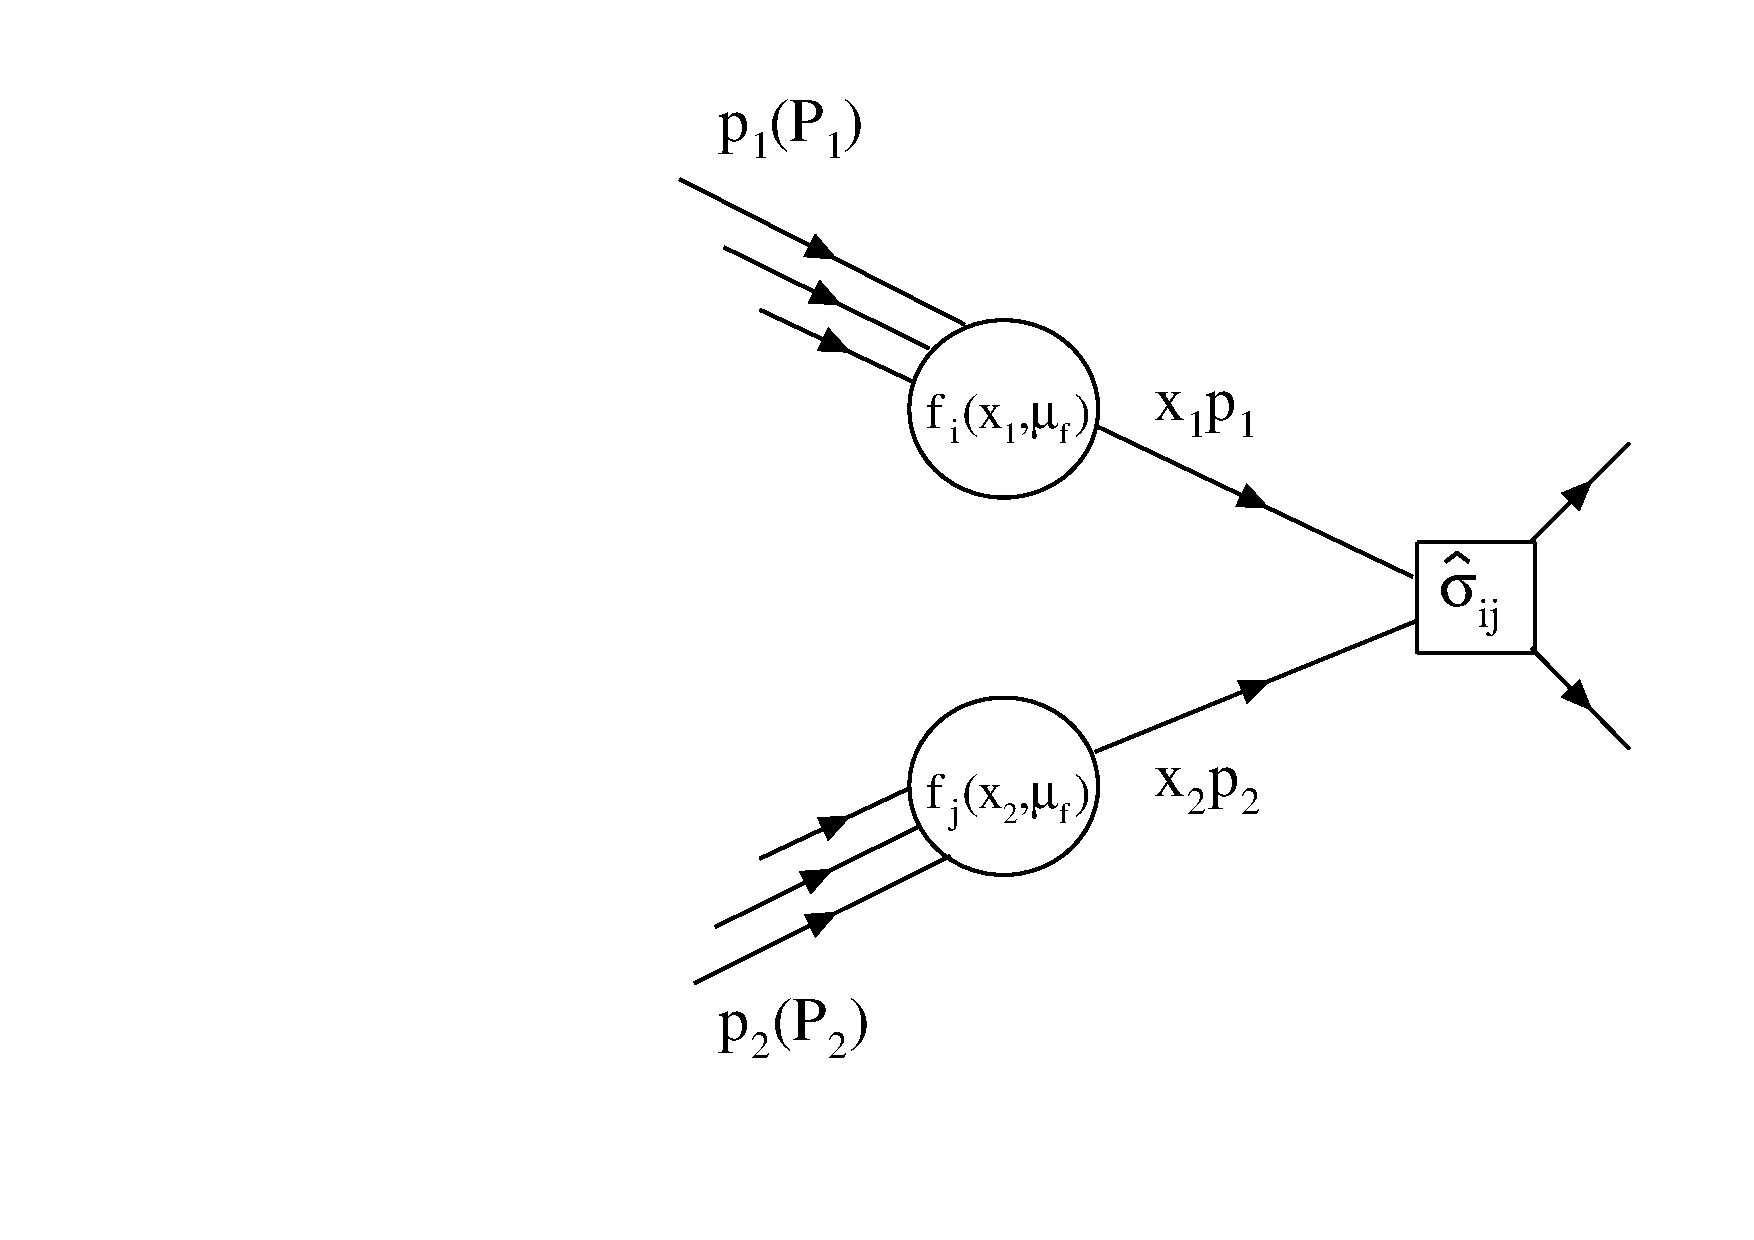
\includegraphics[width=0.65\textwidth]{/home/anter/Desktop/Thesis/Figures/Factorization.pdf}\\
\vspace*{4mm}
\caption[Factorization]{Schematic illustration\footnotemark~of factorization theorem in a collision of two hadrons (protons here) leading to a hard-scattering process at a scale $Q^2$. The two partons $x_1$ and $x_2$ participate in hard interaction with momenta $x_1p_1$ and $x_2p_2$, where $p_1$ and $p_2$ are the momenta of the colliding protons $P_1$ and $P_2$, respectively. The total cross-section is factorized into the hard scattering cross-section $\hat\sigma_{ij}$ calculable using perturbative Quantum Chromodynamics and the PDFs $f_i(x_1,\muf)$ and $f_j(x_2,\muf)$ with factorization scale \muf.}
\label{fig:fac}
\end{center}
\end{figure}
The PDFs of the proton are a necessary input to almost all theory predictions for the hadron colliders. The QCD does not predict the parton content of the proton. So the shapes of PDFs are determined in fits to experimental measurements from data of different experiments. The dependence of PDFs on \muf is calculated using the Dokshitzer-Gribov-Lipatov-Altarelli-Parisi (DGLAP) \cite{Gribov:1972ri,Dokshitzer:1977sg,Altarelli:1977zs} equations which use \alps and the RGE as inputs. The knowledge of proton PDFs mainly comes from the Deep Inelastic Scattering (DIS) HERA, fixed target and TEVATRON data. The LHC data has a potential to improve constraints of the PDFs further as done in one of the recent measurements \cite{Sirunyan:2017skj}. There are several groups which determine the PDFs with the differences in the applied minimization method, the phenomenological approaches and the estimation of the uncertainties. The global PDFs are the CTEQ \cite{Dulat:2015mca}, MMHT \cite{Harland-Lang:2014zoa}, NNPDF \cite{Ball:2014uwa}, ABM \cite{Alekhin:2012ig} and HERAPDF \cite{Abramowicz:2015mha} groups at LO, NLO and NNLO.
\footnotetext{Drawn using ROOT}%Source : \url{https://arxiv.org/pdf/1003.0521.pdf}}

\subsection{Parton Shower and Hadronization}
The hard scattering process involves large momentum transfers due to which the partons involved in it get accelerated. These accelerated colored partons emit QCD radiation in the form of gluons with successively lower energy. Unlike the uncharged photons in QED, the gluons themselves carry color charge and hence also emit further gluons. The emmitted gluons in turn splits into $q\bar{q}$ pairs. This leads to a shower of colored partons called the parton shower. The collinear parton splitting described by splitting functions and the soft gluon emissions contibute mainly to parton shower. The parton shower mimics the effect of higher-order corrections to the hard process. These cannot be calculated exactly and are taken into account using the parton shower approximation. The two incoming partons which are constituents of two colliding hadrons can also develop parton showers, commonly known as Initial-State Radiation (ISR). The initial parton showers till they collide to initiate the hard scattering process. The final outgoing partons produced from a hard scattering process undergo parton showering and give rise to Final-State Radiation (FSR). A parton shower terminates when the scale is below the hadronization scale, which is of order 1 GeV.

With the decrease in energy of partons, the coupling constant of QCD \alps evolves and become large. This leads to the confinement of colored quarks and gluons which leads to the formation of color-neutral composite particles called hadrons. This process is known as hadronization. This process takes place at low momentum transfer and hence non-perturbative in nature. Although no exact theory for hadronization is known, the different phenomenological models have been developed to explain the process of hadronization. These are implemented in Monte Carlo event generators to simulate the hadronization process. \PYTHIA~uses the Lund string model while \HERWIG~is based on the cluster fragmentation model. \\\newline
{\bf Lund String Model -} In the Lund string model of hadronization \cite{Andersson:1998tv}, the highest-energy gluons are treated as field lines. Due to the gluon self-interaction, the gluons are attracted to each other and form a narrow tube (or string) of strong color field between a $q\bar{q}$ pair. This model is based on an observation that at distances greater than about a femtometer, the potential energy $V(r)$ of colored quarks grows linearly with the increase in distance betwee them ($r$) as :
\begin{equation}
V(r) = \kappa r
\end{equation}
where $\kappa \sim {\rm GeV/fm^2}$ is the tension of the string connecting the quarks. When the $q$ and $\bar{q}$ move apart, the gluonic string gets stretched between them and its potential energy grows at the expense of their kinetic energy. When the potential energy becomes of the order of hadron masses, the potential energy is so large that the string breaks at some point along its length, creating a new $q\bar{q}$ pair. The two string segments then again stretch and break until all the potential energy gets converted to $q\bar{q}$ pairs. this whole process is illustrated in Fig~\ref{fig:string}. Then $q$ and $\bar{q}$ hadronize into hadrons due to confinement property. \\ \newline
{\bf Cluster Model -} The cluster model of hadronization \cite{Marchesini:1987cf,Webber:1983if} is based on preconfinement property of QCD \cite{Amati:1979fg}. According to this property, at evolution scales $Q_0$ much less than the hard process scale $Q$, the partons in a shower are clustered in colourless groups with an invariant mass distribution, depending on $Q_0$, not on $Q$ and nature of hard process. This model contains two steps : firtsly all gluons split into $q\bar{q}$ pairs at the end of the parton shower and in the second step, a new set of low-mass color-singlet clusters are obtained which decay into either secondary clusters or directly into hadrons. However, this model has problems in dealing with the decay of very massive clusters.

\begin{figure}[!h]
\begin{center}
\hspace*{-4mm}
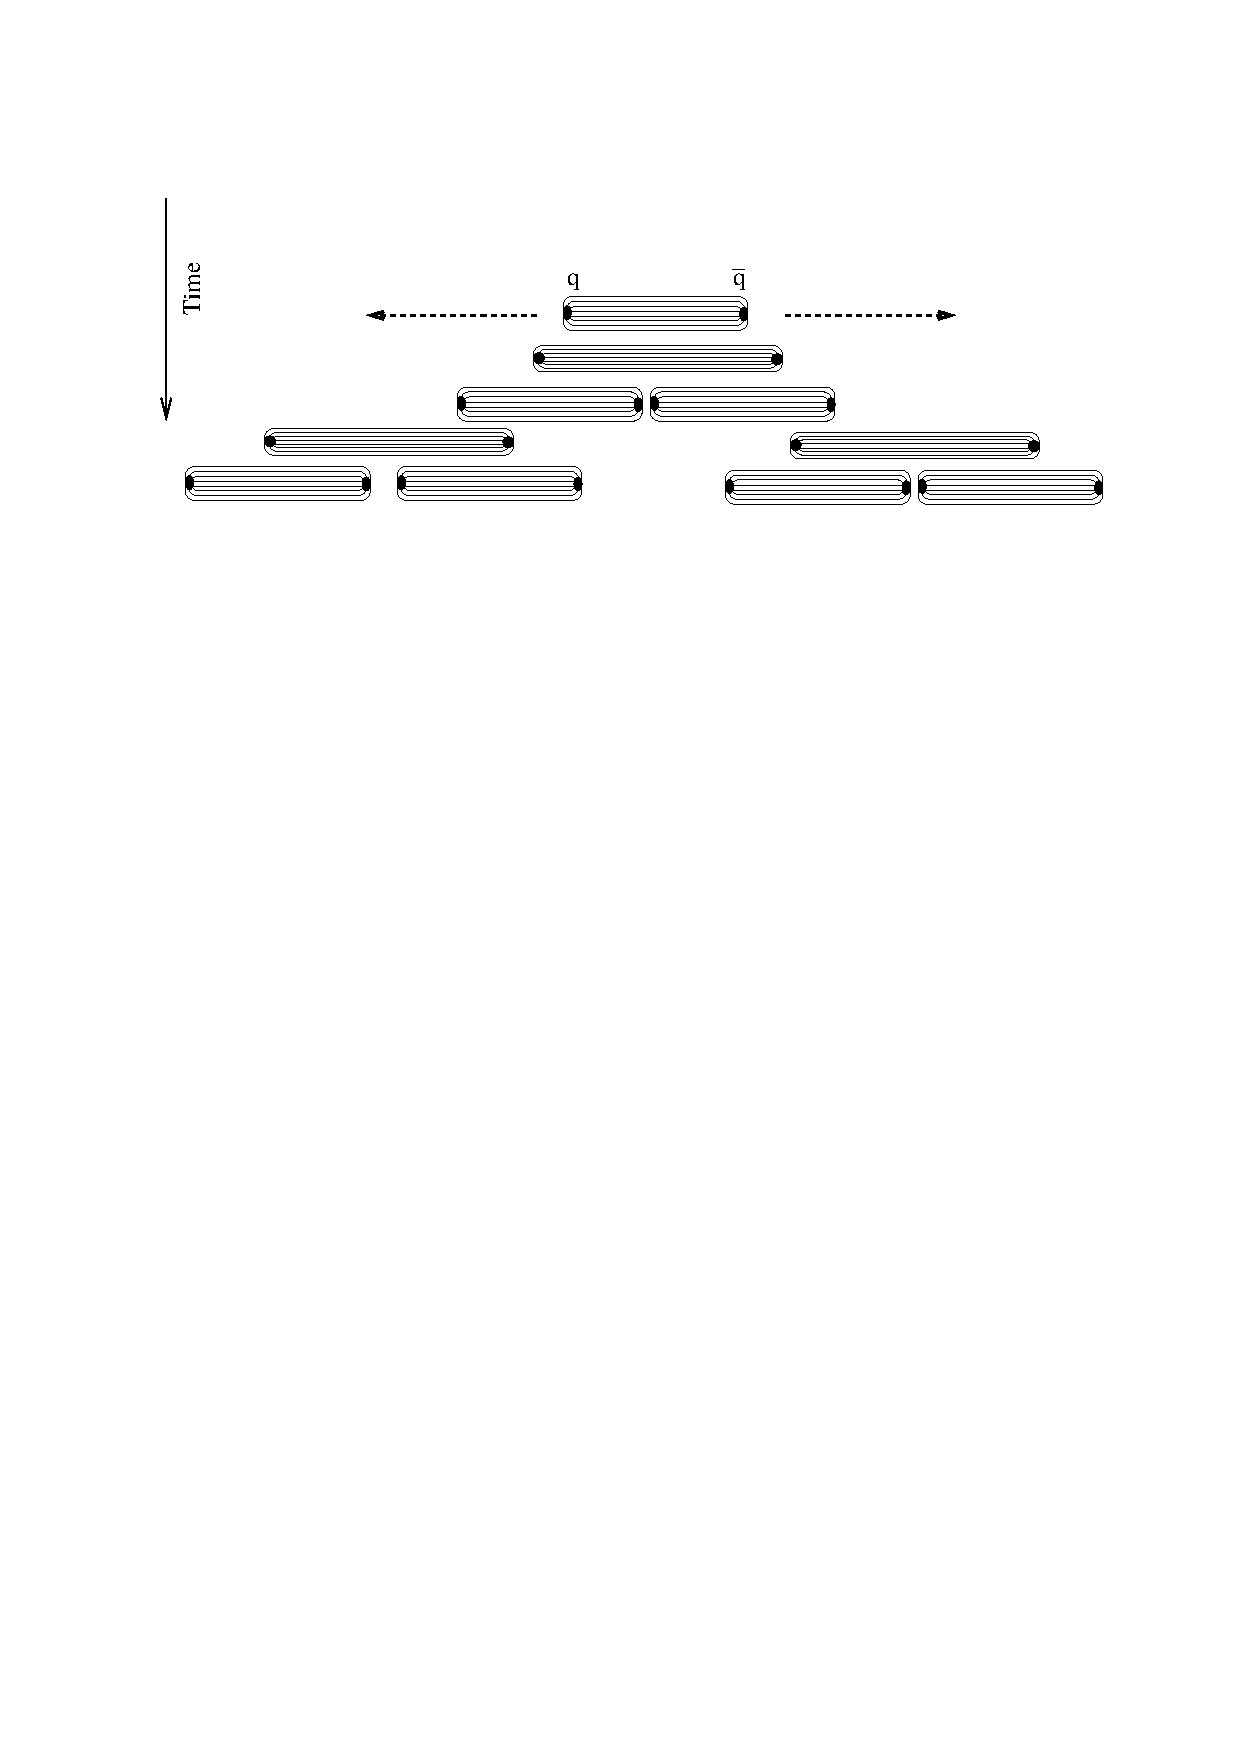
\includegraphics[width=0.95\textwidth]{/home/anter/Desktop/Thesis/Figures/cropped_String.pdf}\\
\vspace*{4mm}
\caption[String]{Illustration of the hadronization process in Lund string model\footnotemark. As the quark $q$ and anti-quark $\bar{q}$ move apart, the potential energy of the gluonic string increases. When it becomes of the order of hadron masses, the string breaks and a new $q\bar{q}$ pair is created. The breaking of string and creation of $q\bar{q}$ continues till all the potential energy gets converted to $q\bar{q}$ pairs which then get hadronized.}
\label{fig:string}
\end{center}
\end{figure}
\footnotetext{Source : \url{http://inspirehep.net/record/806744}}

\subsection{Underlying Event}
In a high energy proton-proton collisons, the underlying event (UE) includes the effects which are not coming from the primary hard scattering process. The UE include the contributions from initial and final-state radiations (ISR, FSR), leftover partons in the collisions called beam remnants and multiple parton interations (MPI). Due to composite nature of proton, the remaining two partons which do not participate in a hard collision, called spectators, may interact giving rise to multiple parton interations. The UE induces an additional energy in the detector which is not related to the main hard interaction. This acts an unavoidable background whose contribution has to be removed because it induces additional energy in the detector not related to the main interaction. There are
several models available for measuring these eects, the most recent one being JIMMY
[20] which is used along with the HERWIG event generator to study p-p collisions at
LHC.

 In a high energy collision of protons, due to the composite physics, the underlying event (UE) is all what is seen in a hadron collider event which is not coming from the primary hard scattering (high energy, high momentum impact) process.[1]


Due to composite nature of proton, the remaining two partons which do not participate in a hard collision, may 
Collectively termed as Underlying Event (UE), the soft activity may receive contributions
from initial and final state radiation (ISR, FSR), leftover partons in the collisions called beam
remnants, and the MPI mentioned above. 


In high energy proton-proton (pp) collisions at LHC, due to the composite nature of
protons, it is possible to have two or more distinct hard parton-parton interactions
occuring simultaneously in a single pp collision.

In hadron collider events that contain a hard subprocess, there is extra hadron production that cannot be ascribed to showering from the coloured partons participating in the subprocess. Furthermore this extra activity, known as the underlying event is greater than that in so-called minimum-bias events, i.e. collisions that do not yield an identifiable hard subprocess. The underlying event is believed to arise from collisions between those partons in the incoming hadrons that do not directly participate in the hard subprocess.
Multiple parton interactions

The most common hard subprocess at a high-energy hadron collider, such as the LHC, is elastic gluon-gluon scattering, gg→gg . The leading-order differential cross section for this subprocess diverges at zero momentum transfer, due to the exchange of a massless virtual gluon. This divergence is presumably regularized below some momentum transfer tmin by higher-order and non-perturbative effects. Nevertheless, for reasonable values of tmin the integrated gluon-gluon scattering cross section is very large, larger even than the total proton-proton scattering cross section. This result is not absurd: it simply indicates that the average number of gluon-gluon collisions per proton-proton collisions is greater than one. Including the cross sections for elastic scattering of quarks, antiquarks and gluons in all possible combinations, all of which diverge in leading order, we see that multiple parton interactions, each with relatively small momentum transfer, are highly probable in hadron-hadron collisions. This is the basis on which modern event generators model both minimum-bias collisions and the underlying event. To account for the extra hadron production when a hard subprocess is present, an event generator must model the impact parameter structure of hadron-hadron collisions. The partons in each incoming hadron are distributed over a transverse area of the order of 1 fm2. The impact parameter of a collision is the transverse distance between the centroids of these areas before the collision. When the impact parameter is large, the areas overlap little and the collision is peripheral, with a low probability of a hard parton-parton interaction and few multiple interactions. On the other hand at small impact parameter the collision is central, with a large overlap, several multiple interactions and a higher probability of a hard interaction. Thus the presence of a hard subprocess is correlated with more multiple interactions and a higher level of underlying event activity. 




The UE is a very important component in a hadronic collision, including most of the occurring
partonic interactions; it can be easily represented as everything that happens in the collision, but
the hard scattering. This general definition stems from the fact that it includes all the different el-
ements which underlie (as the name suggests) the primary hard interaction. In particular, different
subphenomena are grouped under the name of the UE:
• Initial- and final-state radiation which includes the emission of additional particles by partons
in the initial or in the final state, namely before or after the hard scattering;
• Beam-beam remnants (BBR) which group the colour interactions undergone by the spectator
partons in each of the two colliding hadrons;
• Multiple parton interactions (MPI) which contain the whole of additional interactions be-
tween partons of the colliding hadrons, occurring together with the hard scattering.

\begin{figure}[!h]
\begin{center}
\hspace*{-7mm}
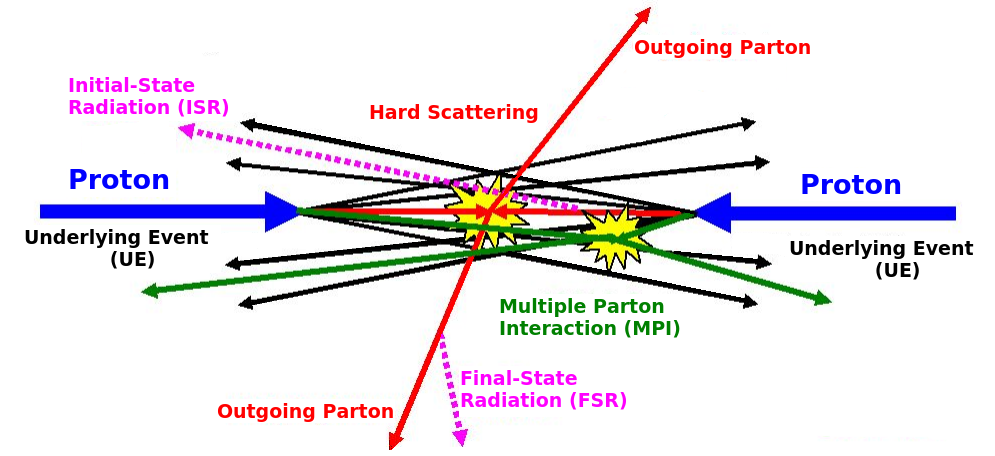
\includegraphics[width=0.95\textwidth]{/home/anter/Desktop/Thesis/Figures/MPI.png}\\
\vspace*{4mm}
\caption[Factorization]{Schematic illustration\footnotemark~of factorization theorem in a collision of two hadrons (protons here) leading to a hard-scattering process at a scale $Q^2$. The two partons $x_1$ and $x_2$ participate in hard interaction with momenta $x_1p_1$ and $x_2p_2$, where $p_1$ and $p_2$ are the momenta of the colliding protons $P_1$ and $P_2$, respectively. The total cross section is factorized into the hard scattering cross section $\hat\sigma_{ij}$ calculable using perturbative Quantum Chromodynamics and the PDFs $f_i(x_1,\muf)$ and $f_j(x_2,\muf)$ with factorization scale \muf.}
\label{fig:MPI}
\end{center}
\end{figure}
\footnotetext{Source : \href{https://www-cdf.fnal.gov/physics/new/qcd/ue_escan/}{The Energy Dependence of Min-Bias and the Underlying Event at CDF}}

\section{Jets}
\label{sec:jets}
Since the partons can not exist as free
particles and can therefore not be measured directly by the experiments, information about
the dynamics of the partons has to be obtained from particle jets produced by the partons
in the scattering process.

\subsection{Jet Algorithms}
\label{sec:jet_algos}
\subsection{Jet Production Cross-Section}

\subsection{Jet Properties}
\begin{comment}
\section{Leading order and next-to-leading order calculations}

A perturbative expansion in $\alpha_{s}$ is generally performed to calculate
measurable quantities in QCD. Physical quantities are calculated 
by separating processes at different orders in $\alpha_{s}$.
At leading order only two jets can exist. Calculations at LO allow for
only 
$gg \rightarrow gg$,
$qq \rightarrow qq$, 
$qg \rightarrow qg$,
$q\bar{q} \rightarrow q\bar{q}$,
$q\bar{q} \rightarrow gg$, and
$gg \rightarrow q\bar{q}$.
Figure shows some of the diagrams which
contribute to leading order parton-parton scattering.
Each vertex in these diagrams is proportional to $\alpha_{s}$. Since 
each diagram at LO has two vertices, calculations can only be performed
at order O($\alpha^{2}_{s}$).
Typically leading order calculations depend heavily upon the choice
of renormalization scale, leading to uncertainties in most LO calculations
of about 30\%.
In order to reduce the theoretical uncertainties, 
higher order diagrams can be introduced. 
As more terms are included in the perturbative expansion, 
the dependence on $\mu$ decreases, reducing the theoretical uncertainties.

At next-to-leading order, calculations may include three 
jet events, because diagrams such as $gg \rightarrow ggg$ are now possible. 
NLO must also include a larger number of two jet diagrams arising from loops.
Figure \ref{FIG:nlo_diagrams} shows some of the diagrams contributing to
NLO parton-parton scattering.
At NLO, each diagram has either three or four vertices, allowing
calculations of order O($\alpha^{3}_{s}$) to be performed. 
Terms which are of order O($\alpha^{4}_{s}$) are ignored.
NLO is much less sensitive to the renormalization scale. Calculations at this
order typically have errors of $\sim$ 10\%. 
 
Calculating quantities to all orders in $\alpha_{s}$
is the ultimate goal. However, it becomes increasingly
difficult to calculate higher order processes. 
At NLO, calculations require over 100 separate diagrams.
The number of diagrams necessary
to calculate higher order corrections is large and the mathematics and computing
time is foreboding. Currently only exact NLO calculations are available.


\begin{comment}
\section{Jet Production}
The high-energy phenomenon involving quantum chromodynamics (QCD) is discussed commonly in terms of quarks and gluons. The property of confinement is responsible for the production of jets in high energy collisions of hadrons. According to the Heisenberg uncertainty principle, the beams with high momentum probe the small distance within the hadron. At high energy, a single parton gets probed within each incoming hadron. So the collision between two hadrons is visualized as a collision between two quarks or two gluons or a quark and a gluon. A quark or a gluon is never visible as after the collision, it begins to get separated from the rest of partons. With the increase in distance, the strength of the force of interaction increases and there is enough energy to create a particle-antiparticle pair. This process continues which leads to the formation of the stable hadrons collimated in the form of bunches. This results in the formation of the jets - spray of hadronic particles. Jets are the final structures observed in the detector. By measuring their energy and direction, we can get close to the original ``parton''. The jet definitions or algorithms are needed to precisely define the jets. The evolution of a jet is illustrated in Figure \ref{ev_j}. A parton that has not yet undergone fragmentation is sometimes referred to as a parton level jet.
A moving parton will radiate gluons and create quark-antiquark pairs by fragmentation and the resulting spray of partons is usually referred to as a parton cascade. The coloured particles within such a cascade
are combined into colourless hadrons through a process called hadronization. The shower
of produced hadrons is usually referred to as a particle level jet.
A jet reconstructed from the energy deposited in a calorimeter by a
particle level jet is referred to as a calorimeter level jet.

\begin{figure}[h!]
\begin{center} 
\includegraphics[scale = 0.75]{figs/Theoretical/jet.pdf}
\caption{Evolution of a jet.}
\label{ev_j}
\end{center}
\end{figure} 
 
\section{Jet Algorithms}
Jet algorithms provide a set of rules for grouping the particles into jets. They usually involve one or more parameters that indicate how close two particles must be for them to belong to the same jet. They can either measure closeness in coordinate space (cone algorithms) or in momentum space (sequential algorithms). They should be able to operate on parton, particle and calorimeter levels. They are always associated with a recombination scheme, to indicate what momentum is assigned to the combined particles. A jet algorithm with its parameters and a recombination scheme forms a ``jet definition''. 
Several important properties that should be met by a jet definition are ~\cite{S.D.} :\\
1. Simple to implement in an experimental analysis;\\
2. Simple to implement in the theoretical calculation;\\
3. Defined at any order of perturbation theory;\\
4. Yields finite cross section at any order of perturbation theory;\\
5. Yields a cross section that is relatively intensive to hadronization.\\

The basic jet kinematics is as following :
The coordinate system is shown in Figure \ref{coordsysI} where r is the radial distance, $\phi$ is the azimuthal angle such that $\phi$ = 0 points to the +x-axis and $\phi$ = $\pi$/2 to the y-axis, and $\theta$ is the polar angle such that $\theta$ = 0 corresponds to +z-axis and $\theta$ = $\pi$ to the -z-axis.

\begin{figure}[h!]
\begin{center} 
\includegraphics[scale = 0.75]{figs/Theoretical/coordinate.jpeg} 
\caption{The coordinate system showing the polar angle ($\theta$), radial
distance (r) and azimuthal angle ($\phi$).}
\label{coordsysI}
\end{center}
\end{figure}

For a fixed particle mass, a relativistically invariant phase space volume d$\tau$ for a particle of momentum $\vec {p}$ and energy E is given by
\begin{equation}
d\tau = \frac {d^3p}{E} = \frac {dp_xdp_ydp_z}{E}
\end{equation} 
Taking z as the collision axis, neither E nor $p_{z}$ are invariant Lorentz transformation. The variables for a suitable choice for analysis is ($P_{T},y,\phi,m$) where $P_{T}$ is transverse momentum to $\hat{z}$ direction, $\phi$ is azimuthal angle about $\hat{z}$, m is mass and $\emph{y}$ is rapidity defined as :
\begin{equation}
y = \frac{1}{2}ln\frac{(E + p_z)}{(E - p_z)}
\end{equation}
For particles with p $\gg$ m = $\sqrt{E^2 - p^2}$,\\
\begin{equation}
y \approx -ln(tan(\theta /2)) \equiv \eta
\end{equation}
where $\eta$ is pseudo-rapidity.\\
P$_{T}$ is always defined in terms of the 3-momentum $\vec{p}$ as 
\begin{equation}
P_{T} = \bf {p}\sin\theta
\end{equation}
The transverse energy $E_{T}$ is given by
 \begin{equation}
E = E_{T}\cosh y
\end{equation}
or
 \begin{equation}
p_z = E_{T}\sinh y
\end{equation}
where 
\begin{equation}
p_z = E\tanh y
\end{equation}

The kinematic properties of the jets (P$_{T}$,$\eta$,$\phi$) can be associated to that of the original partons produced and these are directly measurable.


\subsection{Collinear safety}
Collinear safety is the property by virtue of which the set of hard jets found in the event should not be changed on modification of the event by a collinear splitting i.e. replacement of one parton by two at the same place. An algorithm should be collinear safe. The output of the jet algorithm remains the same if the energy of a particle is distributed among two collinear particles and the collinear singularities should not appear in the perturbative calculations. Two pictures shown in Figure \ref{coll}
 should always produce a single jet. Algorithms which produce zero or two jets (in case of left picture)
are not collinear safe. 
 
\begin{figure}[h!]
\begin{center} 
\includegraphics[scale = 0.55]{figs/Theoretical/collinear_safe.png}
\caption{An example of collinear unsafe behavior of jet algorithm is shown. The right
picture shows the situation if the algorithm constructs one jet. In the left picture due to radiation effect if one jet splits up into two parts. In this worst case no jet
would be produced by seeded algorithm, as both small jets would fall below the threshold.}
\label{coll}
\end{center}
\end{figure}

\subsection{Infrared safety}
Infrared safety is the property due to which the addition of a soft emission i.e. addition of a soft gluon should not change or modify the set of hard jets found in the event. The algorithm should be infrared safe. Along with this, it should also find solutions which are insensitive to soft radiation in the event. The algorithms which look for jets around seeds only can be sensitive to soft radiation as shown in Figure \ref{infra1}. With a soft
gluon emission in the middle of two cone jets, this could lead to overlap
of the two initial cones.
 
\begin{figure}[h!]
\begin{center} 
\includegraphics[scale = 0.55]{figs/Theoretical/infrared_safe.png}
\caption{ Infrared unsafe behavior of jet algorithm is illustrated that how the presence of soft radiation between two jets may cause a merging of the jets that would not occur in the absence of the soft radiation.}
\label{infra1}
\end{center}
\end{figure} 


The motivation behind constructing the jets is to view the events in a way which is insensitive to these effects. The details of various algorithms is given below.

\subsection{Cone algorithms}
In the cone algorithm ~\cite{RunII}, the jet is defined as a cone with fixed radius in $\eta-\phi$ space drawn around the highest energy seed. The set of initial particles over a P$_{T}$ threshold or the midpoints between the previous stable cones can be taken as seeds. The jets are defined as dominant directions of energy flow. The algorithm iterates until the cone is stable which means that the direction of sum of momentum of all the particles is same as that of the center of cone. If we consider the 3-particle event as shown in Figure \ref{infra} and clustering is done using midpoint cone algorithm, 2 stable cones are found leading to 2 jets, shown in (a). If a soft gluon is added to this hard event as shown in figure(b), a third stable cone is found. This change the jet structure on addition of a soft particle and makes the algorithm infrared unsafe. This algorithm is also not collinear safe. 

\begin{figure}[h!]
\begin{center} 
\includegraphics[scale = 1.10]{figs/Theoretical/infraf.png}
\caption{ Stable cones found by the midpoint algorithm for a 3-particle event (left) and for
the same event with an additional infinitely soft gluon (right).}
\label{infra}
\end{center}
\end{figure} 

\subsection{Seedless Infrared-Safe cone (SIS-Cone) algorithm}
The Seedless Infrared-Safe cone (SIS-Cone) algorithm ~\cite{Sis} is an exact seedless cone algorithm that probably identifies all stable cones. It does not rely on seed threshold and it is infrared and collinear safe. This is a complex approach which tests the stability of all subsets of particles and has a complexity of order N$2^{N}$ for N particles, much slower than that of order $N^{3}$ of the midpoint algorithm thus making it unusable for experimental purposes. But this can be reduced to order of $N^{2}$logN ~\cite{Sis} thus making it faster than the midpoint algorithm. 

\subsection{Sequential algorithms}
The sequential algorithm works by defining a distance between pairs of particles and recombining the pair of closest particles successively. This algorithm stops when all the resulting objects are far apart. This is collinear and infrared safe algorithm. It is 
possible for jet cones to overlap such that one particle is contained in more than one jet but the sequential algorithm never 
assigns a particle to more than one jet. The algorithms belonging to this class are:

\subsubsection{$k_{T}$ -algorithm}
The longitudinally invariant $k_{T}$ jet finder ~\cite{Kt1,Kt2} is the most widely used clustering jet finder for proton-(anti)proton collisions. It allows a well defined comparison to the theoretical predictions. 
By restricting ourselves to the approximation that particles are massless, we will have a look at the kinematic variables used 
to represent particle momenta and distances between them. A particle momentum vector {k}, in polar coordinates can be represented as,
\begin{equation}
\vec{k} = (k_{x},k_{y},k_{z}) = \frac {E}{c} \times (\sin\theta\cos\phi,\sin\theta\sin\phi, \cos\theta), 
\end{equation}

where E denotes the particle's energy and taking the incoming particles along the $\pm$z direction.\\
The kinematic properties : transverse momentum $k_{t}$ = $\sqrt{k_{x}^{2} + k_{y}^{2}}$ and the azimuthal angle $\phi$ are longitudinally 
invariant whereas the polar angle transforms in a complicated manner so a quantity called pseudo-rapidity is used,\\
\begin{equation}
\eta = -ln(tan(\theta/2)) 
\end{equation}
In the $k_{T}$ jet finder, the distance measure is 
\begin{equation}
d_{ij} = min(k_{t,i}^{2},k_{t,j}^{2}) \frac{\Delta R_{ij}^{2}}{R^{2}}, \hspace{2 cm} \Delta R_{ij}^{2} = (\eta_i -\eta_j)^{2} + (\phi_i -\phi_j)^{2},
\end{equation}
where $k_{t,i}, \eta_i,\phi_i$ are the transverse momentum, pseudo-rapidity and azimuthal angle of particle i and R is jet-radius parameter,\\
and the particle-beam distance is 
\begin{equation}
d_{iB} = k_{t,i}^{2}.
\end{equation}

Procedure for clustering the particles into jets is as follows:
\begin{itemize}
\item
 Calculate the distance $d_{ij}$ for each pair of particles i and j and distance $d_{iB}$ for each parton i.
\item 
Find the minimum $d_{min}$ of all the $d_{ij},d_{iB}$.
\item
 If $d_{min}$ is $d_{ij}$ then merge the particles i and j into a new single particle k ,summing their ``four-momenta'' by recombination scheme and go to step 1. 
\item
 If $d_{min}$ is $d_{iB}$ , declare particle i to be a final-state jet and remove it from the list. 
\item 
Go to step 1.\\
\end{itemize}

The procedure continues until no particles are left. This is an inclusive mode of clustering. In an exclusive mode of clustering,
 the difference is that the clustering is terminated when all $d_{ij}$,$d_{iB}$ are above the quantity $d_{cut}$ given by $d_{cut} = y_\mathrm{cut}p_{T}^{2}$(jet), where $y_\mathrm{cut}$ is the dimensionless resolution parameter.


\subsubsection{Cambridge/Aachen algorithm}
The formulation of the Cambridge/Aachen algorithm ~\cite{Camb} is similar to that of 
the $k_{T}$ jet algorithm with the difference that the inter-particle distance measure is 

\begin{equation}
d_{ij} = \frac{\Delta R_{ij}^{2}}{R^{2}}, \hspace{2 cm} \Delta R_{ij}^{2} = (\eta_i -\eta_j)^{2} + (\phi_i -\phi_j)^{2},
\end{equation}

and the particle-beam distance is 
\begin{equation}
d_{iB} = 1.
\end{equation}

To extract the jets from the Cambridge/Aachen algorithm exclusively with a $d_{cut}$ parameter, the clustering 
continues up to point where all $d_{ij},d_{iB} > d_{cut}$.

The distance measures can be generalized for the algorithms as : 

\begin{equation}
d_{ij} = min(k_{t,i}^{2p},k_{t,j}^{2p}) \frac{\Delta R_{ij}^{2}}{R^{2}}, \hspace{2 cm} \Delta R_{ij}^{2} = (\eta_i -\eta_j)^{2} + (\phi_i -\phi_j)^{2},
\end{equation}
\begin{equation}
d_{iB} = k_{t,i}^{2p}
\end{equation}

where parameter $\emph{p}$ = 1 for the $k_{T}$ algorithm, 0 for the Cambridge/Aachen algorithm and -1 for the 
anti-$k_{T}$ algorithm ~\cite{AntiKt}. These algorithms are included in the FastJet Package ~\cite{FastJet,FastJet1,FastJet2}, which is used to cluster the particles into jets in a much faster way. The clustering by $k_{T}$ algorithm involves soft particles and that by anti-$k_{T}$ algorithm involves hard particles whereas the Cambridge/Aachen algorithm involves energy independent clusterings. In the anti-$k_{T}$ algorithm, a collinear branching gets clustered at the beginning of the sequence making it collinear and infra-red safe and thus a good substitute for the cone-type algorithms. The $k_{T}$ and the Cambridge/Aachen algorithms give irregular jets but the anti-$k_{T}$ algorithm gives circular hard jets.

\subsection{Recombination Schemes}
A jet algorithm must specify how to combine different partons or particles into a single four-vector. The most widely used recombination scheme is the E-scheme ~\cite{RunII}, or 4-vector recombination scheme which simply adds the four vectors. This has been given as a standard in ~\cite{RunII}. This was the main scheme in use during RUN II of the Tevatron. It is the default option in FastJet ~\cite{FastJet} and is currently used by the LHC experiments. We have also used this in the present work. This scheme calculates the 4-momentum
 of the jet from the 4-momentum of the individual constituents by adding the four-vectors of merging particles i.e. $E = \sum E^{i}, k_{t,x,y,z} = \sum k_{t,x,y,z}^{i}$ where the summation is over all the particles of the jet.
The various recombination schemes have been used experimentally. They differ in the way in which the resolution variables are defined after two particles have been merged into a single one. The data is insensitive to which scheme is used. 
The different types of recombination schemes are :
\begin{itemize}
\item
E$\_$scheme
\item
pt$\_$scheme
\item
pt2$\_$scheme
\item
Et$\_$scheme
\item
Et2$\_$scheme
\item
BIpt$\_$scheme
\item
BIpt2$\_$scheme
\end{itemize}

The p$_{t}$, p$_{t}^{2}$, E$_{t}$ and E$_{t}^{2}$ schemes involve a preprocessing stage to make the initial momenta massless. In the preprocessing stage, re-scaling is done to the energy to be equal to the 3-momentum for the p$_{t}$ and p$_{t}^{2}$ schemes and re-scaling is done to the 3-momentum to be equal to the energy in the E$_{t}$ and E$_{t}^{2}$ schemes. For all the four schemes, the recombined p$_{r}$ of p$_{i}$ and p$_{j}$ is a massless 4-vector which satisfies 
\begin{equation}
p_{t,r} = p_{t,i} + p_{t,j}\\
\end{equation}
\begin{equation}
\phi_{r} = (w_{i}\phi_{i} + w_{j}\phi_{j})/(w_{i} + w_{j})\\
\end{equation}
\begin{equation}
y_{r} = (w_{i}y_{i} + w_{j}y_{j})/(w_{i} + w_{j})\\
\end{equation}
where $\emph{w}_{i}$ is $\emph{p}_{t,i}$ for the p$_{t}$ and E$_{t}$ schemes, and is $\emph{p}_{t,i}^{2}$ for the p$_{t}^{2}$ and E$_{t}^{2}$ schemes. $\emph{p}_{t,i}$, $\phi_{i}$, $\emph{y}_{i}$ are the transverse momentum, azimuthal angle and rapidity of particle i respectively.
As these schemes are not longitudinally invariant for the massive particles, BIpt$\_$scheme and BIpt2$\_$scheme are available. They are identical to the normal p$_{t}$ and p$_{t}^{2}$ schemes with the difference that they do not involve the preprocessing stage.

\section{Subjets}
The internal structure of jets provides an insight into the transition between partons produced in the hard scattering process and the experimentally observable jets of hadrons. The substructure of jets is expected to mainly depend on the type of primary parton, quark or gluon, and the particular hard scattering process but to a lesser extent. The substructure of jets can be studied in terms of the integrated jet shape, $\psi$(r),and the differential jet shape, $\rho$(r), where the energy flow inside a jet is considered, and the subjet multiplicity, <${n_{subj}}$>, where subjets (jet-like structures) within a given jet are studied. The subjets in a particular jet are defined by re-running the jet algorithm only on the particles assigned to a jet .

Unlike for the $k_{T}$ and the Cambridge/Aachen algorithms, 
the anti-$k_{T}$ recombination sequence will slowly expand through a soft subjet, rather than first constructing the soft subjet and then recombining it with a hard subjet. The anti-k$_{T}$ jet algorithm is also a sequential recombination algorithm which merges the particles with high relative P$_{T}$ into jets. So the soft particles within the size R of a high P$_{T}$ jet will be merged with it. So it is less sensitive to details of the distribution of softer objects in an event (or within jets) as it starts clustering with the hardest (highest p$_{T}$) objects in an event. Hence it is less well suited for an investigation of jet substructure. So the clustering sequence inside an anti-$k_{T}$ jet is not usefully related to QCD 
branching.

With k$_{T}$ algorithm, the clustering of the particles in a jet is terminated when all $d_{ij}$,$d_{iB}$ are above the quantity $d_{cut}$ given by $d_{cut} = y_\mathrm{cut}p_{T}^{2}$(jet) ~\cite{dcut}, where $y_\mathrm{cut}$ is the dimensionless resolution parameter such that 0$\leq y_\mathrm{cut} \leq$1 and $p_{T}$(jet) is the transverse momentum of the jet. The parameter $y_\mathrm{cut}$ defines the minimal relative transverse energy between subjets inside the jet and thus determines the extent up-to which the internal jet structure can be resolved. 
In Cambridge/Aachen algorithm, after clustering with some given value of R, the constituents of a particular jet can be clustered into subjets by re-running the algorithm at a smaller radius, $R_{eff}$ = $\sqrt{d_{cut}}$R.
\end{comment}
